
% Default to the notebook output style

    


% Inherit from the specified cell style.




    
\documentclass[11pt]{article}

    
    
    \usepackage[T1]{fontenc}
    % Nicer default font (+ math font) than Computer Modern for most use cases
    \usepackage{mathpazo}

    % Basic figure setup, for now with no caption control since it's done
    % automatically by Pandoc (which extracts ![](path) syntax from Markdown).
    \usepackage{graphicx}
    % We will generate all images so they have a width \maxwidth. This means
    % that they will get their normal width if they fit onto the page, but
    % are scaled down if they would overflow the margins.
    \makeatletter
    \def\maxwidth{\ifdim\Gin@nat@width>\linewidth\linewidth
    \else\Gin@nat@width\fi}
    \makeatother
    \let\Oldincludegraphics\includegraphics
    % Set max figure width to be 80% of text width, for now hardcoded.
    \renewcommand{\includegraphics}[1]{\Oldincludegraphics[width=.8\maxwidth]{#1}}
    % Ensure that by default, figures have no caption (until we provide a
    % proper Figure object with a Caption API and a way to capture that
    % in the conversion process - todo).
    \usepackage{caption}
    \DeclareCaptionLabelFormat{nolabel}{}
    \captionsetup{labelformat=nolabel}

    \usepackage{adjustbox} % Used to constrain images to a maximum size 
    \usepackage{xcolor} % Allow colors to be defined
    \usepackage{enumerate} % Needed for markdown enumerations to work
    \usepackage{geometry} % Used to adjust the document margins
    \usepackage{amsmath} % Equations
    \usepackage{amssymb} % Equations
    \usepackage{textcomp} % defines textquotesingle
    % Hack from http://tex.stackexchange.com/a/47451/13684:
    \AtBeginDocument{%
        \def\PYZsq{\textquotesingle}% Upright quotes in Pygmentized code
    }
    \usepackage{upquote} % Upright quotes for verbatim code
    \usepackage{eurosym} % defines \euro
    \usepackage[mathletters]{ucs} % Extended unicode (utf-8) support
    \usepackage[utf8x]{inputenc} % Allow utf-8 characters in the tex document
    \usepackage{fancyvrb} % verbatim replacement that allows latex
    \usepackage{grffile} % extends the file name processing of package graphics 
                         % to support a larger range 
    % The hyperref package gives us a pdf with properly built
    % internal navigation ('pdf bookmarks' for the table of contents,
    % internal cross-reference links, web links for URLs, etc.)
    \usepackage{hyperref}
    \usepackage{longtable} % longtable support required by pandoc >1.10
    \usepackage{booktabs}  % table support for pandoc > 1.12.2
    \usepackage[inline]{enumitem} % IRkernel/repr support (it uses the enumerate* environment)
    \usepackage[normalem]{ulem} % ulem is needed to support strikethroughs (\sout)
                                % normalem makes italics be italics, not underlines
    

    
    
    % Colors for the hyperref package
    \definecolor{urlcolor}{rgb}{0,.145,.698}
    \definecolor{linkcolor}{rgb}{.71,0.21,0.01}
    \definecolor{citecolor}{rgb}{.12,.54,.11}

    % ANSI colors
    \definecolor{ansi-black}{HTML}{3E424D}
    \definecolor{ansi-black-intense}{HTML}{282C36}
    \definecolor{ansi-red}{HTML}{E75C58}
    \definecolor{ansi-red-intense}{HTML}{B22B31}
    \definecolor{ansi-green}{HTML}{00A250}
    \definecolor{ansi-green-intense}{HTML}{007427}
    \definecolor{ansi-yellow}{HTML}{DDB62B}
    \definecolor{ansi-yellow-intense}{HTML}{B27D12}
    \definecolor{ansi-blue}{HTML}{208FFB}
    \definecolor{ansi-blue-intense}{HTML}{0065CA}
    \definecolor{ansi-magenta}{HTML}{D160C4}
    \definecolor{ansi-magenta-intense}{HTML}{A03196}
    \definecolor{ansi-cyan}{HTML}{60C6C8}
    \definecolor{ansi-cyan-intense}{HTML}{258F8F}
    \definecolor{ansi-white}{HTML}{C5C1B4}
    \definecolor{ansi-white-intense}{HTML}{A1A6B2}

    % commands and environments needed by pandoc snippets
    % extracted from the output of `pandoc -s`
    \providecommand{\tightlist}{%
      \setlength{\itemsep}{0pt}\setlength{\parskip}{0pt}}
    \DefineVerbatimEnvironment{Highlighting}{Verbatim}{commandchars=\\\{\}}
    % Add ',fontsize=\small' for more characters per line
    \newenvironment{Shaded}{}{}
    \newcommand{\KeywordTok}[1]{\textcolor[rgb]{0.00,0.44,0.13}{\textbf{{#1}}}}
    \newcommand{\DataTypeTok}[1]{\textcolor[rgb]{0.56,0.13,0.00}{{#1}}}
    \newcommand{\DecValTok}[1]{\textcolor[rgb]{0.25,0.63,0.44}{{#1}}}
    \newcommand{\BaseNTok}[1]{\textcolor[rgb]{0.25,0.63,0.44}{{#1}}}
    \newcommand{\FloatTok}[1]{\textcolor[rgb]{0.25,0.63,0.44}{{#1}}}
    \newcommand{\CharTok}[1]{\textcolor[rgb]{0.25,0.44,0.63}{{#1}}}
    \newcommand{\StringTok}[1]{\textcolor[rgb]{0.25,0.44,0.63}{{#1}}}
    \newcommand{\CommentTok}[1]{\textcolor[rgb]{0.38,0.63,0.69}{\textit{{#1}}}}
    \newcommand{\OtherTok}[1]{\textcolor[rgb]{0.00,0.44,0.13}{{#1}}}
    \newcommand{\AlertTok}[1]{\textcolor[rgb]{1.00,0.00,0.00}{\textbf{{#1}}}}
    \newcommand{\FunctionTok}[1]{\textcolor[rgb]{0.02,0.16,0.49}{{#1}}}
    \newcommand{\RegionMarkerTok}[1]{{#1}}
    \newcommand{\ErrorTok}[1]{\textcolor[rgb]{1.00,0.00,0.00}{\textbf{{#1}}}}
    \newcommand{\NormalTok}[1]{{#1}}
    
    % Additional commands for more recent versions of Pandoc
    \newcommand{\ConstantTok}[1]{\textcolor[rgb]{0.53,0.00,0.00}{{#1}}}
    \newcommand{\SpecialCharTok}[1]{\textcolor[rgb]{0.25,0.44,0.63}{{#1}}}
    \newcommand{\VerbatimStringTok}[1]{\textcolor[rgb]{0.25,0.44,0.63}{{#1}}}
    \newcommand{\SpecialStringTok}[1]{\textcolor[rgb]{0.73,0.40,0.53}{{#1}}}
    \newcommand{\ImportTok}[1]{{#1}}
    \newcommand{\DocumentationTok}[1]{\textcolor[rgb]{0.73,0.13,0.13}{\textit{{#1}}}}
    \newcommand{\AnnotationTok}[1]{\textcolor[rgb]{0.38,0.63,0.69}{\textbf{\textit{{#1}}}}}
    \newcommand{\CommentVarTok}[1]{\textcolor[rgb]{0.38,0.63,0.69}{\textbf{\textit{{#1}}}}}
    \newcommand{\VariableTok}[1]{\textcolor[rgb]{0.10,0.09,0.49}{{#1}}}
    \newcommand{\ControlFlowTok}[1]{\textcolor[rgb]{0.00,0.44,0.13}{\textbf{{#1}}}}
    \newcommand{\OperatorTok}[1]{\textcolor[rgb]{0.40,0.40,0.40}{{#1}}}
    \newcommand{\BuiltInTok}[1]{{#1}}
    \newcommand{\ExtensionTok}[1]{{#1}}
    \newcommand{\PreprocessorTok}[1]{\textcolor[rgb]{0.74,0.48,0.00}{{#1}}}
    \newcommand{\AttributeTok}[1]{\textcolor[rgb]{0.49,0.56,0.16}{{#1}}}
    \newcommand{\InformationTok}[1]{\textcolor[rgb]{0.38,0.63,0.69}{\textbf{\textit{{#1}}}}}
    \newcommand{\WarningTok}[1]{\textcolor[rgb]{0.38,0.63,0.69}{\textbf{\textit{{#1}}}}}
    
    
    % Define a nice break command that doesn't care if a line doesn't already
    % exist.
    \def\br{\hspace*{\fill} \\* }
    % Math Jax compatability definitions
    \def\gt{>}
    \def\lt{<}
    % Document parameters
    \title{Circuit Analysis Using Sympy\\Assignment 7}
	\author{M V A Suhas Kumar,EE17B109}
    
    
    

    % Pygments definitions
    
\makeatletter
\def\PY@reset{\let\PY@it=\relax \let\PY@bf=\relax%
    \let\PY@ul=\relax \let\PY@tc=\relax%
    \let\PY@bc=\relax \let\PY@ff=\relax}
\def\PY@tok#1{\csname PY@tok@#1\endcsname}
\def\PY@toks#1+{\ifx\relax#1\empty\else%
    \PY@tok{#1}\expandafter\PY@toks\fi}
\def\PY@do#1{\PY@bc{\PY@tc{\PY@ul{%
    \PY@it{\PY@bf{\PY@ff{#1}}}}}}}
\def\PY#1#2{\PY@reset\PY@toks#1+\relax+\PY@do{#2}}

\expandafter\def\csname PY@tok@w\endcsname{\def\PY@tc##1{\textcolor[rgb]{0.73,0.73,0.73}{##1}}}
\expandafter\def\csname PY@tok@c\endcsname{\let\PY@it=\textit\def\PY@tc##1{\textcolor[rgb]{0.25,0.50,0.50}{##1}}}
\expandafter\def\csname PY@tok@cp\endcsname{\def\PY@tc##1{\textcolor[rgb]{0.74,0.48,0.00}{##1}}}
\expandafter\def\csname PY@tok@k\endcsname{\let\PY@bf=\textbf\def\PY@tc##1{\textcolor[rgb]{0.00,0.50,0.00}{##1}}}
\expandafter\def\csname PY@tok@kp\endcsname{\def\PY@tc##1{\textcolor[rgb]{0.00,0.50,0.00}{##1}}}
\expandafter\def\csname PY@tok@kt\endcsname{\def\PY@tc##1{\textcolor[rgb]{0.69,0.00,0.25}{##1}}}
\expandafter\def\csname PY@tok@o\endcsname{\def\PY@tc##1{\textcolor[rgb]{0.40,0.40,0.40}{##1}}}
\expandafter\def\csname PY@tok@ow\endcsname{\let\PY@bf=\textbf\def\PY@tc##1{\textcolor[rgb]{0.67,0.13,1.00}{##1}}}
\expandafter\def\csname PY@tok@nb\endcsname{\def\PY@tc##1{\textcolor[rgb]{0.00,0.50,0.00}{##1}}}
\expandafter\def\csname PY@tok@nf\endcsname{\def\PY@tc##1{\textcolor[rgb]{0.00,0.00,1.00}{##1}}}
\expandafter\def\csname PY@tok@nc\endcsname{\let\PY@bf=\textbf\def\PY@tc##1{\textcolor[rgb]{0.00,0.00,1.00}{##1}}}
\expandafter\def\csname PY@tok@nn\endcsname{\let\PY@bf=\textbf\def\PY@tc##1{\textcolor[rgb]{0.00,0.00,1.00}{##1}}}
\expandafter\def\csname PY@tok@ne\endcsname{\let\PY@bf=\textbf\def\PY@tc##1{\textcolor[rgb]{0.82,0.25,0.23}{##1}}}
\expandafter\def\csname PY@tok@nv\endcsname{\def\PY@tc##1{\textcolor[rgb]{0.10,0.09,0.49}{##1}}}
\expandafter\def\csname PY@tok@no\endcsname{\def\PY@tc##1{\textcolor[rgb]{0.53,0.00,0.00}{##1}}}
\expandafter\def\csname PY@tok@nl\endcsname{\def\PY@tc##1{\textcolor[rgb]{0.63,0.63,0.00}{##1}}}
\expandafter\def\csname PY@tok@ni\endcsname{\let\PY@bf=\textbf\def\PY@tc##1{\textcolor[rgb]{0.60,0.60,0.60}{##1}}}
\expandafter\def\csname PY@tok@na\endcsname{\def\PY@tc##1{\textcolor[rgb]{0.49,0.56,0.16}{##1}}}
\expandafter\def\csname PY@tok@nt\endcsname{\let\PY@bf=\textbf\def\PY@tc##1{\textcolor[rgb]{0.00,0.50,0.00}{##1}}}
\expandafter\def\csname PY@tok@nd\endcsname{\def\PY@tc##1{\textcolor[rgb]{0.67,0.13,1.00}{##1}}}
\expandafter\def\csname PY@tok@s\endcsname{\def\PY@tc##1{\textcolor[rgb]{0.73,0.13,0.13}{##1}}}
\expandafter\def\csname PY@tok@sd\endcsname{\let\PY@it=\textit\def\PY@tc##1{\textcolor[rgb]{0.73,0.13,0.13}{##1}}}
\expandafter\def\csname PY@tok@si\endcsname{\let\PY@bf=\textbf\def\PY@tc##1{\textcolor[rgb]{0.73,0.40,0.53}{##1}}}
\expandafter\def\csname PY@tok@se\endcsname{\let\PY@bf=\textbf\def\PY@tc##1{\textcolor[rgb]{0.73,0.40,0.13}{##1}}}
\expandafter\def\csname PY@tok@sr\endcsname{\def\PY@tc##1{\textcolor[rgb]{0.73,0.40,0.53}{##1}}}
\expandafter\def\csname PY@tok@ss\endcsname{\def\PY@tc##1{\textcolor[rgb]{0.10,0.09,0.49}{##1}}}
\expandafter\def\csname PY@tok@sx\endcsname{\def\PY@tc##1{\textcolor[rgb]{0.00,0.50,0.00}{##1}}}
\expandafter\def\csname PY@tok@m\endcsname{\def\PY@tc##1{\textcolor[rgb]{0.40,0.40,0.40}{##1}}}
\expandafter\def\csname PY@tok@gh\endcsname{\let\PY@bf=\textbf\def\PY@tc##1{\textcolor[rgb]{0.00,0.00,0.50}{##1}}}
\expandafter\def\csname PY@tok@gu\endcsname{\let\PY@bf=\textbf\def\PY@tc##1{\textcolor[rgb]{0.50,0.00,0.50}{##1}}}
\expandafter\def\csname PY@tok@gd\endcsname{\def\PY@tc##1{\textcolor[rgb]{0.63,0.00,0.00}{##1}}}
\expandafter\def\csname PY@tok@gi\endcsname{\def\PY@tc##1{\textcolor[rgb]{0.00,0.63,0.00}{##1}}}
\expandafter\def\csname PY@tok@gr\endcsname{\def\PY@tc##1{\textcolor[rgb]{1.00,0.00,0.00}{##1}}}
\expandafter\def\csname PY@tok@ge\endcsname{\let\PY@it=\textit}
\expandafter\def\csname PY@tok@gs\endcsname{\let\PY@bf=\textbf}
\expandafter\def\csname PY@tok@gp\endcsname{\let\PY@bf=\textbf\def\PY@tc##1{\textcolor[rgb]{0.00,0.00,0.50}{##1}}}
\expandafter\def\csname PY@tok@go\endcsname{\def\PY@tc##1{\textcolor[rgb]{0.53,0.53,0.53}{##1}}}
\expandafter\def\csname PY@tok@gt\endcsname{\def\PY@tc##1{\textcolor[rgb]{0.00,0.27,0.87}{##1}}}
\expandafter\def\csname PY@tok@err\endcsname{\def\PY@bc##1{\setlength{\fboxsep}{0pt}\fcolorbox[rgb]{1.00,0.00,0.00}{1,1,1}{\strut ##1}}}
\expandafter\def\csname PY@tok@kc\endcsname{\let\PY@bf=\textbf\def\PY@tc##1{\textcolor[rgb]{0.00,0.50,0.00}{##1}}}
\expandafter\def\csname PY@tok@kd\endcsname{\let\PY@bf=\textbf\def\PY@tc##1{\textcolor[rgb]{0.00,0.50,0.00}{##1}}}
\expandafter\def\csname PY@tok@kn\endcsname{\let\PY@bf=\textbf\def\PY@tc##1{\textcolor[rgb]{0.00,0.50,0.00}{##1}}}
\expandafter\def\csname PY@tok@kr\endcsname{\let\PY@bf=\textbf\def\PY@tc##1{\textcolor[rgb]{0.00,0.50,0.00}{##1}}}
\expandafter\def\csname PY@tok@bp\endcsname{\def\PY@tc##1{\textcolor[rgb]{0.00,0.50,0.00}{##1}}}
\expandafter\def\csname PY@tok@fm\endcsname{\def\PY@tc##1{\textcolor[rgb]{0.00,0.00,1.00}{##1}}}
\expandafter\def\csname PY@tok@vc\endcsname{\def\PY@tc##1{\textcolor[rgb]{0.10,0.09,0.49}{##1}}}
\expandafter\def\csname PY@tok@vg\endcsname{\def\PY@tc##1{\textcolor[rgb]{0.10,0.09,0.49}{##1}}}
\expandafter\def\csname PY@tok@vi\endcsname{\def\PY@tc##1{\textcolor[rgb]{0.10,0.09,0.49}{##1}}}
\expandafter\def\csname PY@tok@vm\endcsname{\def\PY@tc##1{\textcolor[rgb]{0.10,0.09,0.49}{##1}}}
\expandafter\def\csname PY@tok@sa\endcsname{\def\PY@tc##1{\textcolor[rgb]{0.73,0.13,0.13}{##1}}}
\expandafter\def\csname PY@tok@sb\endcsname{\def\PY@tc##1{\textcolor[rgb]{0.73,0.13,0.13}{##1}}}
\expandafter\def\csname PY@tok@sc\endcsname{\def\PY@tc##1{\textcolor[rgb]{0.73,0.13,0.13}{##1}}}
\expandafter\def\csname PY@tok@dl\endcsname{\def\PY@tc##1{\textcolor[rgb]{0.73,0.13,0.13}{##1}}}
\expandafter\def\csname PY@tok@s2\endcsname{\def\PY@tc##1{\textcolor[rgb]{0.73,0.13,0.13}{##1}}}
\expandafter\def\csname PY@tok@sh\endcsname{\def\PY@tc##1{\textcolor[rgb]{0.73,0.13,0.13}{##1}}}
\expandafter\def\csname PY@tok@s1\endcsname{\def\PY@tc##1{\textcolor[rgb]{0.73,0.13,0.13}{##1}}}
\expandafter\def\csname PY@tok@mb\endcsname{\def\PY@tc##1{\textcolor[rgb]{0.40,0.40,0.40}{##1}}}
\expandafter\def\csname PY@tok@mf\endcsname{\def\PY@tc##1{\textcolor[rgb]{0.40,0.40,0.40}{##1}}}
\expandafter\def\csname PY@tok@mh\endcsname{\def\PY@tc##1{\textcolor[rgb]{0.40,0.40,0.40}{##1}}}
\expandafter\def\csname PY@tok@mi\endcsname{\def\PY@tc##1{\textcolor[rgb]{0.40,0.40,0.40}{##1}}}
\expandafter\def\csname PY@tok@il\endcsname{\def\PY@tc##1{\textcolor[rgb]{0.40,0.40,0.40}{##1}}}
\expandafter\def\csname PY@tok@mo\endcsname{\def\PY@tc##1{\textcolor[rgb]{0.40,0.40,0.40}{##1}}}
\expandafter\def\csname PY@tok@ch\endcsname{\let\PY@it=\textit\def\PY@tc##1{\textcolor[rgb]{0.25,0.50,0.50}{##1}}}
\expandafter\def\csname PY@tok@cm\endcsname{\let\PY@it=\textit\def\PY@tc##1{\textcolor[rgb]{0.25,0.50,0.50}{##1}}}
\expandafter\def\csname PY@tok@cpf\endcsname{\let\PY@it=\textit\def\PY@tc##1{\textcolor[rgb]{0.25,0.50,0.50}{##1}}}
\expandafter\def\csname PY@tok@c1\endcsname{\let\PY@it=\textit\def\PY@tc##1{\textcolor[rgb]{0.25,0.50,0.50}{##1}}}
\expandafter\def\csname PY@tok@cs\endcsname{\let\PY@it=\textit\def\PY@tc##1{\textcolor[rgb]{0.25,0.50,0.50}{##1}}}

\def\PYZbs{\char`\\}
\def\PYZus{\char`\_}
\def\PYZob{\char`\{}
\def\PYZcb{\char`\}}
\def\PYZca{\char`\^}
\def\PYZam{\char`\&}
\def\PYZlt{\char`\<}
\def\PYZgt{\char`\>}
\def\PYZsh{\char`\#}
\def\PYZpc{\char`\%}
\def\PYZdl{\char`\$}
\def\PYZhy{\char`\-}
\def\PYZsq{\char`\'}
\def\PYZdq{\char`\"}
\def\PYZti{\char`\~}
% for compatibility with earlier versions
\def\PYZat{@}
\def\PYZlb{[}
\def\PYZrb{]}
\makeatother


    % Exact colors from NB
    \definecolor{incolor}{rgb}{0.0, 0.0, 0.5}
    \definecolor{outcolor}{rgb}{0.545, 0.0, 0.0}



    
    % Prevent overflowing lines due to hard-to-break entities
    \sloppy 
    % Setup hyperref package
    \hypersetup{
      breaklinks=true,  % so long urls are correctly broken across lines
      colorlinks=true,
      urlcolor=urlcolor,
      linkcolor=linkcolor,
      citecolor=citecolor,
      }
    % Slightly bigger margins than the latex defaults
    
    \geometry{verbose,tmargin=1in,bmargin=1in,lmargin=1in,rmargin=1in}
    
    

    \begin{document}
    
    
    \maketitle
    
    \section{Introduction}\label{introduction}

In this assignment, we use Sympy to analytically solve a matrix equation
governing an analog circuit. We look at two circuits, an active low pass
filter and an active high pass filter. We create matrices using node
equations for the circuits in sympy, and then solve the equations
analytically. We then convert the resulting sympy solution into a numpy
function which can be called. We then use the signals toolbox we studied
in the last assignment to understand the responses of the two circuits
to various inputs.

    Importing required packages

    \begin{Verbatim}[commandchars=\\\{\}]
{\color{incolor}In [{\color{incolor}1}]:} \PY{k+kn}{from} \PY{n+nn}{sympy} \PY{k}{import} \PY{o}{*}
        \PY{k+kn}{import} \PY{n+nn}{numpy} \PY{k}{as} \PY{n+nn}{np}
        \PY{k+kn}{import} \PY{n+nn}{matplotlib}\PY{n+nn}{.}\PY{n+nn}{pyplot} \PY{k}{as} \PY{n+nn}{plt}
        \PY{k+kn}{import} \PY{n+nn}{scipy}\PY{n+nn}{.}\PY{n+nn}{signal} \PY{k}{as} \PY{n+nn}{sp}
        \PY{k+kn}{from} \PY{n+nn}{pylab} \PY{k}{import} \PY{o}{*}
        \PY{k+kn}{from} \PY{n+nn}{IPython}\PY{n+nn}{.}\PY{n+nn}{display} \PY{k}{import} \PY{o}{*}
\end{Verbatim}


    \section{Low pass Filter}\label{low-pass-filter}

    \begin{figure}
\centering
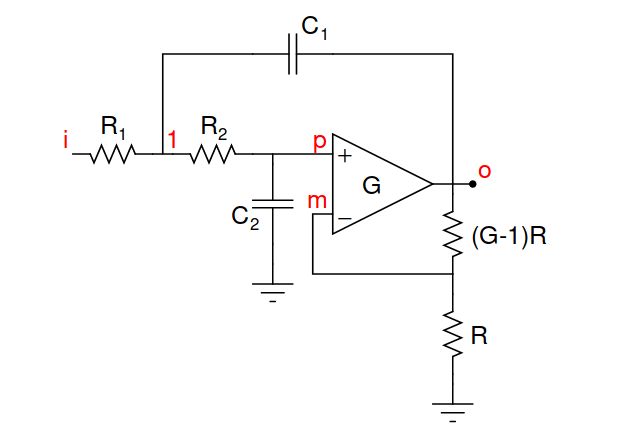
\includegraphics{circuit1.png}
\caption{Circuit1}
\end{figure}

    where G =1.586 and R1 = R2 = 10kΩ and C1=C2=10pF. This gives a 3dB
Butter-worth filter with cutoff frequency of 1/2πMHz.

Circuit Equations are as follows: \[V_{m}=\frac{V_{o}}{G}\]\\
\[ V_{p} =V_{1} \frac{1}{1+s R_{2}C_{2}}\] \[ V_{o} = G(V_{p} - V_{m})\]
\[\frac{V_{i}-V_{1}}{R_{1}} + \frac{V_{p}-V_{1}}{R_{2}} + s C_{1}(V_{0}-V_{1}) = 0\]
Solving the above equations with approxmtion gives

\[ V_{o} \approx \frac{V_{i}}{s R_{1} C_{1}}\]

We would like to solve this in Python and also get (and plot) the exact
result. For this we need the sympy module.

    To solve the equtions exactly we use matrix method of solving:

    \begin{Verbatim}[commandchars=\\\{\}]
{\color{incolor}In [{\color{incolor}2}]:} \PY{n}{init\PYZus{}printing}\PY{p}{(}\PY{p}{)}
        \PY{n}{R1}\PY{p}{,}\PY{n}{R2}\PY{p}{,}\PY{n}{C1}\PY{p}{,}\PY{n}{C2}\PY{p}{,}\PY{n}{G} \PY{o}{=} \PY{n}{symbols}\PY{p}{(}\PY{l+s+s2}{\PYZdq{}}\PY{l+s+s2}{R1 R2 C1 C2 G}\PY{l+s+s2}{\PYZdq{}}\PY{p}{)}
        \PY{n}{V1}\PY{p}{,}\PY{n}{Vp}\PY{p}{,}\PY{n}{Vm}\PY{p}{,}\PY{n}{Vo}\PY{p}{,}\PY{n}{Vi} \PY{o}{=} \PY{n}{symbols}\PY{p}{(}\PY{l+s+s2}{\PYZdq{}}\PY{l+s+s2}{V1 Vp Vm Vo Vi}\PY{l+s+s2}{\PYZdq{}}\PY{p}{)}
        \PY{n}{s} \PY{o}{=} \PY{n}{symbols}\PY{p}{(}\PY{l+s+s2}{\PYZdq{}}\PY{l+s+s2}{s}\PY{l+s+s2}{\PYZdq{}}\PY{p}{)}
        \PY{n}{A} \PY{o}{=} \PY{n}{Matrix}\PY{p}{(}\PY{p}{[}\PY{p}{[}\PY{l+m+mi}{0}\PY{p}{,}\PY{l+m+mi}{0}\PY{p}{,}\PY{l+m+mi}{1}\PY{p}{,}\PY{o}{\PYZhy{}}\PY{l+m+mi}{1}\PY{o}{/}\PY{n}{G}\PY{p}{]}\PY{p}{,}
                    \PY{p}{[}\PY{o}{\PYZhy{}}\PY{l+m+mi}{1}\PY{o}{/}\PY{p}{(}\PY{l+m+mi}{1}\PY{o}{+}\PY{n}{s}\PY{o}{*}\PY{n}{R2}\PY{o}{*}\PY{n}{C2}\PY{p}{)}\PY{p}{,}\PY{l+m+mi}{1}\PY{p}{,}\PY{l+m+mi}{0}\PY{p}{,}\PY{l+m+mi}{0}\PY{p}{]}\PY{p}{,}
                    \PY{p}{[}\PY{l+m+mi}{0}\PY{p}{,}\PY{o}{\PYZhy{}}\PY{n}{G}\PY{p}{,}\PY{n}{G}\PY{p}{,}\PY{l+m+mi}{1}\PY{p}{]}\PY{p}{,}
                  \PY{p}{[}\PY{o}{\PYZhy{}}\PY{l+m+mi}{1}\PY{o}{/}\PY{n}{R1}\PY{o}{\PYZhy{}}\PY{l+m+mi}{1}\PY{o}{/}\PY{n}{R2}\PY{o}{\PYZhy{}}\PY{n}{s}\PY{o}{*}\PY{n}{C1}\PY{p}{,}\PY{l+m+mi}{1}\PY{o}{/}\PY{n}{R2}\PY{p}{,}\PY{l+m+mi}{0}\PY{p}{,}\PY{n}{s}\PY{o}{*}\PY{n}{C1}\PY{p}{]}\PY{p}{]}\PY{p}{)}
        \PY{n}{M} \PY{o}{=} \PY{n}{Matrix}\PY{p}{(}\PY{p}{[}\PY{n}{V1}\PY{p}{,}\PY{n}{Vp}\PY{p}{,}\PY{n}{Vm}\PY{p}{,}\PY{n}{Vo}\PY{p}{]}\PY{p}{)}
        \PY{n}{b} \PY{o}{=} \PY{n}{Matrix}\PY{p}{(}\PY{p}{[}\PY{l+m+mi}{0}\PY{p}{,}\PY{l+m+mi}{0}\PY{p}{,}\PY{l+m+mi}{0}\PY{p}{,}\PY{n}{Vi}\PY{o}{/}\PY{n}{R1}\PY{p}{]}\PY{p}{)}
        \PY{n}{display}\PY{p}{(}\PY{n}{Eq}\PY{p}{(}\PY{n}{MatMul}\PY{p}{(}\PY{n}{A}\PY{p}{,}\PY{n}{M}\PY{p}{)}\PY{p}{,}\PY{n}{b}\PY{p}{)}\PY{p}{)}
\end{Verbatim}


    $$\left[\begin{matrix}0 & 0 & 1 & - \frac{1}{G}\\- \frac{1}{C_{2} R_{2} s + 1} & 1 & 0 & 0\\0 & - G & G & 1\\- C_{1} s - \frac{1}{R_{2}} - \frac{1}{R_{1}} & \frac{1}{R_{2}} & 0 & C_{1} s\end{matrix}\right] \left[\begin{matrix}V_{1}\\Vp\\Vm\\Vo\end{matrix}\right] = \left[\begin{matrix}0\\0\\0\\\frac{Vi}{R_{1}}\end{matrix}\right]$$

    
    Solving the above matrix yield exact result

    Function defining low pass filter:

    \begin{Verbatim}[commandchars=\\\{\}]
{\color{incolor}In [{\color{incolor}3}]:} \PY{k}{def} \PY{n+nf}{lowpass}\PY{p}{(}\PY{n}{R1}\PY{o}{=}\PY{l+m+mi}{10}\PY{o}{*}\PY{o}{*}\PY{l+m+mi}{4}\PY{p}{,}\PY{n}{R2}\PY{o}{=}\PY{l+m+mi}{10}\PY{o}{*}\PY{o}{*}\PY{l+m+mi}{4}\PY{p}{,}\PY{n}{C1}\PY{o}{=}\PY{l+m+mi}{10}\PY{o}{*}\PY{o}{*}\PY{o}{\PYZhy{}}\PY{l+m+mi}{11}\PY{p}{,}\PY{n}{C2}\PY{o}{=}\PY{l+m+mi}{10}\PY{o}{*}\PY{o}{*}\PY{o}{\PYZhy{}}\PY{l+m+mi}{11}\PY{p}{,}\PY{n}{G}\PY{o}{=}\PY{l+m+mf}{1.586}\PY{p}{,}\PY{n}{Vi}\PY{o}{=}\PY{l+m+mi}{1}\PY{p}{)}\PY{p}{:}
            \PY{n}{s}\PY{o}{=}\PY{n}{symbols}\PY{p}{(}\PY{l+s+s2}{\PYZdq{}}\PY{l+s+s2}{s}\PY{l+s+s2}{\PYZdq{}}\PY{p}{)}
            \PY{n}{A}\PY{o}{=}\PY{n}{Matrix}\PY{p}{(}\PY{p}{[}\PY{p}{[}\PY{l+m+mi}{0}\PY{p}{,}\PY{l+m+mi}{0}\PY{p}{,}\PY{l+m+mi}{1}\PY{p}{,}\PY{o}{\PYZhy{}}\PY{l+m+mi}{1}\PY{o}{/}\PY{n}{G}\PY{p}{]}\PY{p}{,}
                      \PY{p}{[}\PY{o}{\PYZhy{}}\PY{l+m+mi}{1}\PY{o}{/}\PY{p}{(}\PY{l+m+mi}{1}\PY{o}{+}\PY{n}{s}\PY{o}{*}\PY{n}{R2}\PY{o}{*}\PY{n}{C2}\PY{p}{)}\PY{p}{,}\PY{l+m+mi}{1}\PY{p}{,}\PY{l+m+mi}{0}\PY{p}{,}\PY{l+m+mi}{0}\PY{p}{]}\PY{p}{,}
                      \PY{p}{[}\PY{l+m+mi}{0}\PY{p}{,}\PY{o}{\PYZhy{}}\PY{n}{G}\PY{p}{,}\PY{n}{G}\PY{p}{,}\PY{l+m+mi}{1}\PY{p}{]}\PY{p}{,}
                      \PY{p}{[}\PY{o}{\PYZhy{}}\PY{l+m+mi}{1}\PY{o}{/}\PY{n}{R1}\PY{o}{\PYZhy{}}\PY{l+m+mi}{1}\PY{o}{/}\PY{n}{R2}\PY{o}{\PYZhy{}}\PY{n}{s}\PY{o}{*}\PY{n}{C1}\PY{p}{,}\PY{l+m+mi}{1}\PY{o}{/}\PY{n}{R2}\PY{p}{,}\PY{l+m+mi}{0}\PY{p}{,}\PY{n}{s}\PY{o}{*}\PY{n}{C1}\PY{p}{]}\PY{p}{]}\PY{p}{)}
            \PY{n}{b}\PY{o}{=}\PY{n}{Matrix}\PY{p}{(}\PY{p}{[}\PY{l+m+mi}{0}\PY{p}{,}\PY{l+m+mi}{0}\PY{p}{,}\PY{l+m+mi}{0}\PY{p}{,}\PY{n}{Vi}\PY{o}{/}\PY{n}{R1}\PY{p}{]}\PY{p}{)}
            \PY{n}{V} \PY{o}{=} \PY{n}{A}\PY{o}{.}\PY{n}{inv}\PY{p}{(}\PY{p}{)}\PY{o}{*}\PY{n}{b}
            \PY{k}{return}\PY{p}{(}\PY{n}{A}\PY{p}{,}\PY{n}{b}\PY{p}{,}\PY{n}{V}\PY{p}{)}
            
\end{Verbatim}


    Function which can take input in laplace domain or time domain and give
the output of low pass filter:

    \begin{Verbatim}[commandchars=\\\{\}]
{\color{incolor}In [{\color{incolor}4}]:} \PY{k}{def} \PY{n+nf}{low\PYZus{}pass\PYZus{}output}\PY{p}{(}\PY{n}{laplace\PYZus{}fn} \PY{o}{=} \PY{k+kc}{None}\PY{p}{,}\PY{n}{time\PYZus{}fn}\PY{o}{=}\PY{k+kc}{None}\PY{p}{,}\PY{n}{t}\PY{o}{=}\PY{n}{np}\PY{o}{.}\PY{n}{linspace}\PY{p}{(}\PY{l+m+mi}{0}\PY{p}{,}\PY{l+m+mf}{1e\PYZhy{}5}\PY{p}{,}\PY{l+m+mf}{1e5}\PY{p}{)}\PY{p}{,}\PY{n}{C}\PY{o}{=}\PY{l+m+mi}{10}\PY{o}{*}\PY{o}{*}\PY{o}{\PYZhy{}}\PY{l+m+mi}{11}\PY{p}{)}\PY{p}{:}
            \PY{n}{A}\PY{p}{,}\PY{n}{b}\PY{p}{,}\PY{n}{V} \PY{o}{=} \PY{n}{lowpass}\PY{p}{(}\PY{n}{C1}\PY{o}{=}\PY{n}{C}\PY{p}{,}\PY{n}{C2}\PY{o}{=}\PY{n}{C}\PY{p}{)}
            \PY{n}{v\PYZus{}low\PYZus{}pass} \PY{o}{=} \PY{n}{V}\PY{p}{[}\PY{o}{\PYZhy{}}\PY{l+m+mi}{1}\PY{p}{]}
            \PY{n}{temp} \PY{o}{=} \PY{n}{expand}\PY{p}{(}\PY{n}{simplify}\PY{p}{(}\PY{n}{v\PYZus{}low\PYZus{}pass}\PY{p}{)}\PY{p}{)}
            \PY{n}{n}\PY{p}{,}\PY{n}{d} \PY{o}{=} \PY{n}{fraction}\PY{p}{(}\PY{n}{temp}\PY{p}{)}
            \PY{n}{n}\PY{p}{,}\PY{n}{d} \PY{o}{=} \PY{n}{Poly}\PY{p}{(}\PY{n}{n}\PY{p}{,}\PY{n}{s}\PY{p}{)}\PY{p}{,}\PY{n}{Poly}\PY{p}{(}\PY{n}{d}\PY{p}{,}\PY{n}{s}\PY{p}{)}
            \PY{n}{num}\PY{p}{,}\PY{n}{den} \PY{o}{=} \PY{n}{n}\PY{o}{.}\PY{n}{all\PYZus{}coeffs}\PY{p}{(}\PY{p}{)}\PY{p}{,}\PY{n}{d}\PY{o}{.}\PY{n}{all\PYZus{}coeffs}\PY{p}{(}\PY{p}{)}
            \PY{n}{H\PYZus{}v\PYZus{}low\PYZus{}pass} \PY{o}{=} \PY{n}{sp}\PY{o}{.}\PY{n}{lti}\PY{p}{(}\PY{p}{[}\PY{o}{\PYZhy{}}\PY{n+nb}{float}\PY{p}{(}\PY{n}{f}\PY{p}{)} \PY{k}{for} \PY{n}{f} \PY{o+ow}{in} \PY{n}{num}\PY{p}{]}\PY{p}{,}\PY{p}{[}\PY{n+nb}{float}\PY{p}{(}\PY{n}{f}\PY{p}{)} \PY{k}{for} \PY{n}{f} \PY{o+ow}{in} \PY{n}{den}\PY{p}{]}\PY{p}{)}
            \PY{k}{if} \PY{n}{laplace\PYZus{}fn} \PY{o}{!=}\PY{k+kc}{None}\PY{p}{:}
                \PY{n}{temp} \PY{o}{=} \PY{n}{expand}\PY{p}{(}\PY{n}{simplify}\PY{p}{(}\PY{n}{laplace\PYZus{}fn}\PY{p}{)}\PY{p}{)}
                \PY{n}{n}\PY{p}{,}\PY{n}{d} \PY{o}{=} \PY{n}{fraction}\PY{p}{(}\PY{n}{temp}\PY{p}{)}
                \PY{n}{n}\PY{p}{,}\PY{n}{d} \PY{o}{=} \PY{n}{Poly}\PY{p}{(}\PY{n}{n}\PY{p}{,}\PY{n}{s}\PY{p}{)}\PY{p}{,}\PY{n}{Poly}\PY{p}{(}\PY{n}{d}\PY{p}{,}\PY{n}{s}\PY{p}{)}
                \PY{n}{num}\PY{p}{,}\PY{n}{den} \PY{o}{=} \PY{n}{n}\PY{o}{.}\PY{n}{all\PYZus{}coeffs}\PY{p}{(}\PY{p}{)}\PY{p}{,}\PY{n}{d}\PY{o}{.}\PY{n}{all\PYZus{}coeffs}\PY{p}{(}\PY{p}{)}
                \PY{n}{lap} \PY{o}{=} \PY{n}{sp}\PY{o}{.}\PY{n}{lti}\PY{p}{(}\PY{p}{[}\PY{n+nb}{float}\PY{p}{(}\PY{n}{f}\PY{p}{)} \PY{k}{for} \PY{n}{f} \PY{o+ow}{in} \PY{n}{num}\PY{p}{]}\PY{p}{,}\PY{p}{[}\PY{n+nb}{float}\PY{p}{(}\PY{n}{f}\PY{p}{)} \PY{k}{for} \PY{n}{f} \PY{o+ow}{in} \PY{n}{den}\PY{p}{]}\PY{p}{)}
                \PY{n}{t}\PY{p}{,}\PY{n}{u} \PY{o}{=} \PY{n}{sp}\PY{o}{.}\PY{n}{impulse}\PY{p}{(}\PY{n}{lap}\PY{p}{,}\PY{k+kc}{None}\PY{p}{,}\PY{n}{t}\PY{p}{)}
            \PY{k}{else}\PY{p}{:}
                \PY{n}{u} \PY{o}{=} \PY{n}{time\PYZus{}fn}
            \PY{n}{t}\PY{p}{,}\PY{n}{V\PYZus{}out}\PY{p}{,}\PY{n}{svec} \PY{o}{=} \PY{n}{sp}\PY{o}{.}\PY{n}{lsim}\PY{p}{(}\PY{n}{H\PYZus{}v\PYZus{}low\PYZus{}pass}\PY{p}{,}\PY{n}{u}\PY{p}{,}\PY{n}{t}\PY{p}{)}
            \PY{k}{return} \PY{p}{(}\PY{n}{t}\PY{p}{,}\PY{n}{V\PYZus{}out}\PY{p}{)}
\end{Verbatim}


    \begin{Verbatim}[commandchars=\\\{\}]
/home/suhas/anaconda3/lib/python3.6/site-packages/ipykernel\_launcher.py:1: DeprecationWarning: object of type <class 'float'> cannot be safely interpreted as an integer.
  """Entry point for launching an IPython kernel.

    \end{Verbatim}

    \section{High pass filter}\label{high-pass-filter}

    \begin{figure}
\centering
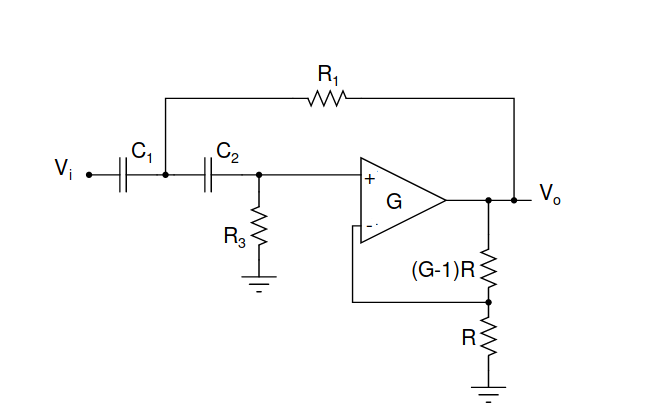
\includegraphics{high.png}
\caption{High pass filter}
\end{figure}

    values you can use are R1=R3=10kΩ, C1=C2=1nF, and G=1.586

Circuit Equations are as follows: \[V_{n}=\frac{V_{o}}{G}\]\\
\[ V_{p} =V_{1} \frac{s R_{3}C_{2}}{1+s R_{3}C_{2}}\]
\[ V_{o} = G(V_{p} - V_{n})\]
\[(V_{1}-V_{i})sC_{1} + \frac{(V_{1}-V_{o})}{R_{1}} + (V_{i}-V_{p})sC_{2} = 0 \]

    \begin{Verbatim}[commandchars=\\\{\}]
{\color{incolor}In [{\color{incolor}5}]:} \PY{n}{R1}\PY{p}{,} \PY{n}{R3}\PY{p}{,} \PY{n}{C1}\PY{p}{,} \PY{n}{C2}\PY{p}{,} \PY{n}{G}\PY{p}{,} \PY{n}{Vi} \PY{o}{=} \PY{n}{symbols}\PY{p}{(}\PY{l+s+s1}{\PYZsq{}}\PY{l+s+s1}{R\PYZus{}1 R\PYZus{}3 C\PYZus{}1 C\PYZus{}2 G V\PYZus{}i}\PY{l+s+s1}{\PYZsq{}}\PY{p}{)}
        \PY{n}{V1}\PY{p}{,}\PY{n}{Vn}\PY{p}{,}\PY{n}{Vp}\PY{p}{,}\PY{n}{Vo} \PY{o}{=} \PY{n}{symbols}\PY{p}{(}\PY{l+s+s1}{\PYZsq{}}\PY{l+s+s1}{V\PYZus{}1 V\PYZus{}n V\PYZus{}p V\PYZus{}o}\PY{l+s+s1}{\PYZsq{}}\PY{p}{)}
        \PY{n}{x}\PY{o}{=}\PY{n}{Matrix}\PY{p}{(}\PY{p}{[}\PY{n}{V1}\PY{p}{,}\PY{n}{Vn}\PY{p}{,}\PY{n}{Vp}\PY{p}{,}\PY{n}{Vo}\PY{p}{]}\PY{p}{)}
        
        \PY{n}{A}\PY{o}{=}\PY{n}{Matrix}\PY{p}{(}\PY{p}{[}\PY{p}{[}\PY{l+m+mi}{0}\PY{p}{,}\PY{o}{\PYZhy{}}\PY{l+m+mi}{1}\PY{p}{,}\PY{l+m+mi}{0}\PY{p}{,}\PY{l+m+mi}{1}\PY{o}{/}\PY{n}{G}\PY{p}{]}\PY{p}{,}
                \PY{p}{[}\PY{n}{s}\PY{o}{*}\PY{n}{C2}\PY{o}{*}\PY{n}{R3}\PY{o}{/}\PY{p}{(}\PY{n}{s}\PY{o}{*}\PY{n}{C2}\PY{o}{*}\PY{n}{R3}\PY{o}{+}\PY{l+m+mi}{1}\PY{p}{)}\PY{p}{,}\PY{l+m+mi}{0}\PY{p}{,}\PY{o}{\PYZhy{}}\PY{l+m+mi}{1}\PY{p}{,}\PY{l+m+mi}{0}\PY{p}{]}\PY{p}{,}
                \PY{p}{[}\PY{l+m+mi}{0}\PY{p}{,}\PY{n}{G}\PY{p}{,}\PY{o}{\PYZhy{}}\PY{n}{G}\PY{p}{,}\PY{l+m+mi}{1}\PY{p}{]}\PY{p}{,}
                \PY{p}{[}\PY{o}{\PYZhy{}}\PY{n}{s}\PY{o}{*}\PY{n}{C2}\PY{o}{\PYZhy{}}\PY{l+m+mi}{1}\PY{o}{/}\PY{n}{R1}\PY{o}{\PYZhy{}}\PY{n}{s}\PY{o}{*}\PY{n}{C1}\PY{p}{,}\PY{l+m+mi}{0}\PY{p}{,}\PY{n}{s}\PY{o}{*}\PY{n}{C2}\PY{p}{,}\PY{l+m+mi}{1}\PY{o}{/}\PY{n}{R1}\PY{p}{]}\PY{p}{]}\PY{p}{)}
        
        \PY{n}{b}\PY{o}{=}\PY{n}{Matrix}\PY{p}{(}\PY{p}{[}\PY{l+m+mi}{0}\PY{p}{,}\PY{l+m+mi}{0}\PY{p}{,}\PY{l+m+mi}{0}\PY{p}{,}\PY{o}{\PYZhy{}}\PY{n}{Vi}\PY{o}{*}\PY{n}{s}\PY{o}{*}\PY{n}{C1}\PY{p}{]}\PY{p}{)}
        \PY{n}{init\PYZus{}printing}
        \PY{n}{display}\PY{p}{(}\PY{n}{Eq}\PY{p}{(}\PY{n}{MatMul}\PY{p}{(}\PY{n}{A}\PY{p}{,}\PY{n}{x}\PY{p}{)}\PY{p}{,}\PY{n}{b}\PY{p}{)}\PY{p}{)}
\end{Verbatim}


    $$\left[\begin{matrix}0 & -1 & 0 & \frac{1}{G}\\\frac{C_{2} R_{3} s}{C_{2} R_{3} s + 1} & 0 & -1 & 0\\0 & G & - G & 1\\- C_{1} s - C_{2} s - \frac{1}{R_{1}} & 0 & C_{2} s & \frac{1}{R_{1}}\end{matrix}\right] \left[\begin{matrix}V_{1}\\V_{n}\\V_{p}\\V_{o}\end{matrix}\right] = \left[\begin{matrix}0\\0\\0\\- C_{1} V_{i} s\end{matrix}\right]$$

    
    Function defining high pass filter:

    \begin{Verbatim}[commandchars=\\\{\}]
{\color{incolor}In [{\color{incolor}6}]:} \PY{k}{def} \PY{n+nf}{highpass}\PY{p}{(}\PY{n}{R1}\PY{o}{=}\PY{l+m+mi}{10}\PY{o}{*}\PY{o}{*}\PY{l+m+mi}{4}\PY{p}{,}\PY{n}{R3}\PY{o}{=}\PY{l+m+mi}{10}\PY{o}{*}\PY{o}{*}\PY{l+m+mi}{4}\PY{p}{,}\PY{n}{C1}\PY{o}{=}\PY{l+m+mi}{10}\PY{o}{*}\PY{o}{*}\PY{o}{\PYZhy{}}\PY{l+m+mi}{9}\PY{p}{,}\PY{n}{C2}\PY{o}{=}\PY{l+m+mi}{10}\PY{o}{*}\PY{o}{*}\PY{o}{\PYZhy{}}\PY{l+m+mi}{9}\PY{p}{,}\PY{n}{G}\PY{o}{=}\PY{l+m+mf}{1.586}\PY{p}{,}\PY{n}{Vi}\PY{o}{=}\PY{l+m+mi}{1}\PY{p}{)}\PY{p}{:}
            \PY{n}{s}\PY{o}{=} \PY{n}{symbols}\PY{p}{(}\PY{l+s+s2}{\PYZdq{}}\PY{l+s+s2}{s}\PY{l+s+s2}{\PYZdq{}}\PY{p}{)}
            \PY{n}{A}\PY{o}{=}\PY{n}{Matrix}\PY{p}{(}\PY{p}{[}\PY{p}{[}\PY{l+m+mi}{0}\PY{p}{,}\PY{o}{\PYZhy{}}\PY{l+m+mi}{1}\PY{p}{,}\PY{l+m+mi}{0}\PY{p}{,}\PY{l+m+mi}{1}\PY{o}{/}\PY{n}{G}\PY{p}{]}\PY{p}{,}
                \PY{p}{[}\PY{n}{s}\PY{o}{*}\PY{n}{C2}\PY{o}{*}\PY{n}{R3}\PY{o}{/}\PY{p}{(}\PY{n}{s}\PY{o}{*}\PY{n}{C2}\PY{o}{*}\PY{n}{R3}\PY{o}{+}\PY{l+m+mi}{1}\PY{p}{)}\PY{p}{,}\PY{l+m+mi}{0}\PY{p}{,}\PY{o}{\PYZhy{}}\PY{l+m+mi}{1}\PY{p}{,}\PY{l+m+mi}{0}\PY{p}{]}\PY{p}{,}
                \PY{p}{[}\PY{l+m+mi}{0}\PY{p}{,}\PY{n}{G}\PY{p}{,}\PY{o}{\PYZhy{}}\PY{n}{G}\PY{p}{,}\PY{l+m+mi}{1}\PY{p}{]}\PY{p}{,}
                \PY{p}{[}\PY{o}{\PYZhy{}}\PY{n}{s}\PY{o}{*}\PY{n}{C2}\PY{o}{\PYZhy{}}\PY{l+m+mi}{1}\PY{o}{/}\PY{n}{R1}\PY{o}{\PYZhy{}}\PY{n}{s}\PY{o}{*}\PY{n}{C1}\PY{p}{,}\PY{l+m+mi}{0}\PY{p}{,}\PY{n}{s}\PY{o}{*}\PY{n}{C2}\PY{p}{,}\PY{l+m+mi}{1}\PY{o}{/}\PY{n}{R1}\PY{p}{]}\PY{p}{]}\PY{p}{)}
        
            \PY{n}{b}\PY{o}{=}\PY{n}{Matrix}\PY{p}{(}\PY{p}{[}\PY{l+m+mi}{0}\PY{p}{,}\PY{l+m+mi}{0}\PY{p}{,}\PY{l+m+mi}{0}\PY{p}{,}\PY{o}{\PYZhy{}}\PY{n}{Vi}\PY{o}{*}\PY{n}{s}\PY{o}{*}\PY{n}{C1}\PY{p}{]}\PY{p}{)}
            \PY{n}{V} \PY{o}{=}\PY{n}{A}\PY{o}{.}\PY{n}{inv}\PY{p}{(}\PY{p}{)} \PY{o}{*} \PY{n}{b}
            \PY{k}{return} \PY{p}{(}\PY{n}{A}\PY{p}{,}\PY{n}{b}\PY{p}{,}\PY{n}{V}\PY{p}{)}
            
\end{Verbatim}


    Function which can take input in laplace domain or time domain and give
the output of high pass filter:

    \begin{Verbatim}[commandchars=\\\{\}]
{\color{incolor}In [{\color{incolor}7}]:} \PY{k}{def} \PY{n+nf}{high\PYZus{}pass\PYZus{}output}\PY{p}{(}\PY{n}{laplace\PYZus{}fn} \PY{o}{=} \PY{k+kc}{None}\PY{p}{,}\PY{n}{time\PYZus{}fn}\PY{o}{=}\PY{k+kc}{None}\PY{p}{,}\PY{n}{t}\PY{o}{=}\PY{n}{np}\PY{o}{.}\PY{n}{linspace}\PY{p}{(}\PY{l+m+mi}{0}\PY{p}{,}\PY{l+m+mf}{1e\PYZhy{}4}\PY{p}{,}\PY{l+m+mf}{1e5}\PY{p}{)}\PY{p}{,}\PY{n}{C}\PY{o}{=}\PY{l+m+mi}{10}\PY{o}{*}\PY{o}{*}\PY{o}{\PYZhy{}}\PY{l+m+mi}{11}\PY{p}{)}\PY{p}{:}
            \PY{n}{A}\PY{p}{,}\PY{n}{b}\PY{p}{,}\PY{n}{V} \PY{o}{=} \PY{n}{highpass}\PY{p}{(}\PY{n}{C1}\PY{o}{=}\PY{n}{C}\PY{p}{,}\PY{n}{C2}\PY{o}{=}\PY{n}{C}\PY{p}{)}
            \PY{n}{v\PYZus{}high\PYZus{}pass} \PY{o}{=} \PY{n}{V}\PY{p}{[}\PY{o}{\PYZhy{}}\PY{l+m+mi}{1}\PY{p}{]}
            \PY{n}{temp} \PY{o}{=} \PY{n}{expand}\PY{p}{(}\PY{n}{simplify}\PY{p}{(}\PY{n}{v\PYZus{}high\PYZus{}pass}\PY{p}{)}\PY{p}{)}
            \PY{n}{n}\PY{p}{,}\PY{n}{d} \PY{o}{=} \PY{n}{fraction}\PY{p}{(}\PY{n}{temp}\PY{p}{)}
            \PY{n}{n}\PY{p}{,}\PY{n}{d} \PY{o}{=} \PY{n}{Poly}\PY{p}{(}\PY{n}{n}\PY{p}{,}\PY{n}{s}\PY{p}{)}\PY{p}{,}\PY{n}{Poly}\PY{p}{(}\PY{n}{d}\PY{p}{,}\PY{n}{s}\PY{p}{)}
            \PY{n}{num}\PY{p}{,}\PY{n}{den} \PY{o}{=} \PY{n}{n}\PY{o}{.}\PY{n}{all\PYZus{}coeffs}\PY{p}{(}\PY{p}{)}\PY{p}{,}\PY{n}{d}\PY{o}{.}\PY{n}{all\PYZus{}coeffs}\PY{p}{(}\PY{p}{)}
            \PY{n}{H\PYZus{}v\PYZus{}high\PYZus{}pass} \PY{o}{=} \PY{n}{sp}\PY{o}{.}\PY{n}{lti}\PY{p}{(}\PY{p}{[}\PY{n+nb}{float}\PY{p}{(}\PY{n}{f}\PY{p}{)} \PY{k}{for} \PY{n}{f} \PY{o+ow}{in} \PY{n}{num}\PY{p}{]}\PY{p}{,}\PY{p}{[}\PY{n+nb}{float}\PY{p}{(}\PY{n}{f}\PY{p}{)} \PY{k}{for} \PY{n}{f} \PY{o+ow}{in} \PY{n}{den}\PY{p}{]}\PY{p}{)}
            \PY{k}{if} \PY{n}{laplace\PYZus{}fn} \PY{o}{!=}\PY{k+kc}{None}\PY{p}{:}
                \PY{n}{temp} \PY{o}{=} \PY{n}{expand}\PY{p}{(}\PY{n}{simplify}\PY{p}{(}\PY{n}{laplace\PYZus{}fn}\PY{p}{)}\PY{p}{)}
                \PY{n}{n}\PY{p}{,}\PY{n}{d} \PY{o}{=} \PY{n}{fraction}\PY{p}{(}\PY{n}{temp}\PY{p}{)}
                \PY{n}{n}\PY{p}{,}\PY{n}{d} \PY{o}{=} \PY{n}{Poly}\PY{p}{(}\PY{n}{n}\PY{p}{,}\PY{n}{s}\PY{p}{)}\PY{p}{,}\PY{n}{Poly}\PY{p}{(}\PY{n}{d}\PY{p}{,}\PY{n}{s}\PY{p}{)}
                \PY{n}{num}\PY{p}{,}\PY{n}{den} \PY{o}{=} \PY{n}{n}\PY{o}{.}\PY{n}{all\PYZus{}coeffs}\PY{p}{(}\PY{p}{)}\PY{p}{,}\PY{n}{d}\PY{o}{.}\PY{n}{all\PYZus{}coeffs}\PY{p}{(}\PY{p}{)}
                \PY{n}{lap} \PY{o}{=} \PY{n}{sp}\PY{o}{.}\PY{n}{lti}\PY{p}{(}\PY{p}{[}\PY{n+nb}{float}\PY{p}{(}\PY{n}{f}\PY{p}{)} \PY{k}{for} \PY{n}{f} \PY{o+ow}{in} \PY{n}{num}\PY{p}{]}\PY{p}{,}\PY{p}{[}\PY{n+nb}{float}\PY{p}{(}\PY{n}{f}\PY{p}{)} \PY{k}{for} \PY{n}{f} \PY{o+ow}{in} \PY{n}{den}\PY{p}{]}\PY{p}{)}
                \PY{n}{t}\PY{p}{,}\PY{n}{u} \PY{o}{=} \PY{n}{sp}\PY{o}{.}\PY{n}{impulse}\PY{p}{(}\PY{n}{lap}\PY{p}{,}\PY{k+kc}{None}\PY{p}{,}\PY{n}{t}\PY{p}{)}
            \PY{k}{else}\PY{p}{:}
                \PY{n}{u} \PY{o}{=} \PY{n}{time\PYZus{}fn}
            \PY{n}{t}\PY{p}{,}\PY{n}{V\PYZus{}out}\PY{p}{,}\PY{n}{svec} \PY{o}{=} \PY{n}{sp}\PY{o}{.}\PY{n}{lsim}\PY{p}{(}\PY{n}{H\PYZus{}v\PYZus{}high\PYZus{}pass}\PY{p}{,}\PY{n}{u}\PY{p}{,}\PY{n}{t}\PY{p}{)}
            \PY{k}{return} \PY{p}{(}\PY{n}{t}\PY{p}{,}\PY{n}{V\PYZus{}out}\PY{p}{)}
\end{Verbatim}


    \begin{Verbatim}[commandchars=\\\{\}]
/home/suhas/anaconda3/lib/python3.6/site-packages/ipykernel\_launcher.py:2: DeprecationWarning: object of type <class 'float'> cannot be safely interpreted as an integer.
  

    \end{Verbatim}

    \section{Question1}\label{question1}

    Step Response for low pass filter

    \begin{Verbatim}[commandchars=\\\{\}]
{\color{incolor}In [{\color{incolor}8}]:} \PY{n}{t}\PY{p}{,}\PY{n}{V\PYZus{}low\PYZus{}step} \PY{o}{=} \PY{n}{low\PYZus{}pass\PYZus{}output}\PY{p}{(}\PY{n}{laplace\PYZus{}fn}\PY{o}{=}\PY{l+m+mi}{1}\PY{o}{/}\PY{n}{s}\PY{p}{)}
\end{Verbatim}


    \begin{Verbatim}[commandchars=\\\{\}]
{\color{incolor}In [{\color{incolor}9}]:} \PY{n}{plt}\PY{o}{.}\PY{n}{plot}\PY{p}{(}\PY{n}{t}\PY{p}{,}\PY{n}{V\PYZus{}low\PYZus{}step}\PY{p}{)}
        \PY{n}{plt}\PY{o}{.}\PY{n}{grid}\PY{p}{(}\PY{k+kc}{True}\PY{p}{)}
        \PY{n}{plt}\PY{o}{.}\PY{n}{xlabel}\PY{p}{(}\PY{l+s+s2}{\PYZdq{}}\PY{l+s+s2}{t \PYZhy{}\PYZhy{}\PYZhy{}\PYZhy{}\PYZhy{}\PYZhy{}\PYZgt{}}\PY{l+s+s2}{\PYZdq{}}\PY{p}{,}\PY{n}{size}\PY{o}{=}\PY{l+m+mi}{14}\PY{p}{)}
        \PY{n}{plt}\PY{o}{.}\PY{n}{ylabel}\PY{p}{(}\PY{l+s+sa}{r}\PY{l+s+s2}{\PYZdq{}}\PY{l+s+s2}{\PYZdl{}Step}\PY{l+s+s2}{\PYZbs{}}\PY{l+s+s2}{ Response}\PY{l+s+s2}{\PYZbs{}}\PY{l+s+s2}{ V\PYZus{}}\PY{l+s+si}{\PYZob{}o\PYZcb{}}\PY{l+s+s2}{(t)\PYZdl{}}\PY{l+s+s2}{\PYZdq{}}\PY{p}{,}\PY{n}{size}\PY{o}{=}\PY{l+m+mi}{14}\PY{p}{)}
        \PY{n}{plt}\PY{o}{.}\PY{n}{title}\PY{p}{(}\PY{l+s+s2}{\PYZdq{}}\PY{l+s+s2}{Step Response When Capacitance = 10pF in low pass filter}\PY{l+s+s2}{\PYZdq{}}\PY{p}{)}
        \PY{n}{plt}\PY{o}{.}\PY{n}{show}\PY{p}{(}\PY{p}{)}
\end{Verbatim}


    \begin{center}
    \adjustimage{max size={0.9\linewidth}{0.9\paperheight}}{output_25_0.png}
    \end{center}
    { \hspace*{\fill} \\}
    
    Step response is starting from zero and reaching 0.793 at steady
state.This is because DC gain oftransfer function is 0.793.Initial value
is 0 because AC gain of low pass filter is zero(impulse can be assumed
as High frequency signal and we know low pass filter dosen't pass high
frequency signal).

    \section{Question2}\label{question2}

    Finding Output when input signal is
\[(sin(2000πt)+cos(2×106πt))u_{o}(t)\]

    \begin{Verbatim}[commandchars=\\\{\}]
{\color{incolor}In [{\color{incolor}10}]:} \PY{n}{t} \PY{o}{=} \PY{n}{np}\PY{o}{.}\PY{n}{linspace}\PY{p}{(}\PY{l+m+mi}{0}\PY{p}{,}\PY{l+m+mf}{1e\PYZhy{}3}\PY{p}{,}\PY{l+m+mf}{1e5}\PY{p}{)}
         \PY{n}{plt}\PY{o}{.}\PY{n}{plot}\PY{p}{(}\PY{n}{t}\PY{p}{,}\PY{n}{np}\PY{o}{.}\PY{n}{sin}\PY{p}{(}\PY{l+m+mi}{2000}\PY{o}{*}\PY{n}{np}\PY{o}{.}\PY{n}{pi}\PY{o}{*}\PY{n}{t}\PY{p}{)}\PY{o}{+}\PY{n}{np}\PY{o}{.}\PY{n}{cos}\PY{p}{(}\PY{l+m+mf}{2e6}\PY{o}{*}\PY{n}{np}\PY{o}{.}\PY{n}{pi}\PY{o}{*}\PY{n}{t}\PY{p}{)}\PY{p}{)}
         \PY{n}{plt}\PY{o}{.}\PY{n}{grid}\PY{p}{(}\PY{k+kc}{True}\PY{p}{)}
         \PY{n}{plt}\PY{o}{.}\PY{n}{xlabel}\PY{p}{(}\PY{l+s+s2}{\PYZdq{}}\PY{l+s+s2}{t \PYZhy{}\PYZhy{}\PYZhy{}\PYZhy{}\PYZhy{}\PYZhy{}\PYZgt{}}\PY{l+s+s2}{\PYZdq{}}\PY{p}{,}\PY{n}{size}\PY{o}{=}\PY{l+m+mi}{14}\PY{p}{)}
         \PY{n}{plt}\PY{o}{.}\PY{n}{ylabel}\PY{p}{(}\PY{l+s+sa}{r}\PY{l+s+s2}{\PYZdq{}}\PY{l+s+s2}{\PYZdl{}V\PYZus{}}\PY{l+s+si}{\PYZob{}i\PYZcb{}}\PY{l+s+s2}{(t)\PYZdl{}}\PY{l+s+s2}{\PYZdq{}}\PY{p}{,}\PY{n}{size}\PY{o}{=}\PY{l+m+mi}{14}\PY{p}{)}
         \PY{n}{plt}\PY{o}{.}\PY{n}{title}\PY{p}{(}\PY{l+s+s2}{\PYZdq{}}\PY{l+s+s2}{Mixed frequency input}\PY{l+s+s2}{\PYZdq{}}\PY{p}{)}
         \PY{n}{plt}\PY{o}{.}\PY{n}{show}\PY{p}{(}\PY{p}{)}
\end{Verbatim}


    \begin{Verbatim}[commandchars=\\\{\}]
/home/suhas/anaconda3/lib/python3.6/site-packages/ipykernel\_launcher.py:1: DeprecationWarning: object of type <class 'float'> cannot be safely interpreted as an integer.
  """Entry point for launching an IPython kernel.

    \end{Verbatim}

    \begin{center}
    \adjustimage{max size={0.9\linewidth}{0.9\paperheight}}{output_29_1.png}
    \end{center}
    { \hspace*{\fill} \\}
    
    Band is high frequency wave and envolope is the low frequency wave

    \begin{Verbatim}[commandchars=\\\{\}]
{\color{incolor}In [{\color{incolor}11}]:} \PY{n}{t} \PY{o}{=} \PY{n}{linspace}\PY{p}{(}\PY{l+m+mi}{0}\PY{p}{,}\PY{l+m+mf}{1e\PYZhy{}5}\PY{p}{,}\PY{l+m+mf}{1e5}\PY{p}{)}
         \PY{n}{t}\PY{p}{,}\PY{n}{vout} \PY{o}{=} \PY{n}{low\PYZus{}pass\PYZus{}output}\PY{p}{(}\PY{n}{time\PYZus{}fn}\PY{o}{=}\PY{n}{np}\PY{o}{.}\PY{n}{sin}\PY{p}{(}\PY{l+m+mi}{2000}\PY{o}{*}\PY{n}{np}\PY{o}{.}\PY{n}{pi}\PY{o}{*}\PY{n}{t}\PY{p}{)}\PY{o}{+}\PY{n}{np}\PY{o}{.}\PY{n}{cos}\PY{p}{(}\PY{l+m+mf}{2e6}\PY{o}{*}\PY{n}{np}\PY{o}{.}\PY{n}{pi}\PY{o}{*}\PY{n}{t}\PY{p}{)}\PY{p}{,}\PY{n}{t}\PY{o}{=}\PY{n}{t}\PY{p}{,}\PY{n}{C}\PY{o}{=}\PY{l+m+mi}{10}\PY{o}{*}\PY{o}{*}\PY{o}{\PYZhy{}}\PY{l+m+mi}{9}\PY{p}{)}
\end{Verbatim}


    \begin{Verbatim}[commandchars=\\\{\}]
/home/suhas/anaconda3/lib/python3.6/site-packages/ipykernel\_launcher.py:2: DeprecationWarning: object of type <class 'float'> cannot be safely interpreted as an integer.
  

    \end{Verbatim}

    \begin{Verbatim}[commandchars=\\\{\}]
{\color{incolor}In [{\color{incolor}12}]:} \PY{n}{plt}\PY{o}{.}\PY{n}{plot}\PY{p}{(}\PY{n}{t}\PY{p}{,}\PY{n}{vout}\PY{p}{)}
         \PY{n}{plt}\PY{o}{.}\PY{n}{grid}\PY{p}{(}\PY{k+kc}{True}\PY{p}{)}
         \PY{n}{plt}\PY{o}{.}\PY{n}{xlabel}\PY{p}{(}\PY{l+s+s2}{\PYZdq{}}\PY{l+s+s2}{t \PYZhy{}\PYZhy{}\PYZhy{}\PYZhy{}\PYZhy{}\PYZhy{}\PYZgt{}}\PY{l+s+s2}{\PYZdq{}}\PY{p}{,}\PY{n}{size}\PY{o}{=}\PY{l+m+mi}{14}\PY{p}{)}
         \PY{n}{plt}\PY{o}{.}\PY{n}{ylabel}\PY{p}{(}\PY{l+s+sa}{r}\PY{l+s+s2}{\PYZdq{}}\PY{l+s+s2}{\PYZdl{}V\PYZus{}}\PY{l+s+si}{\PYZob{}o\PYZcb{}}\PY{l+s+s2}{(t)\PYZdl{}}\PY{l+s+s2}{\PYZdq{}}\PY{p}{,}\PY{n}{size}\PY{o}{=}\PY{l+m+mi}{14}\PY{p}{)}
         \PY{n}{plt}\PY{o}{.}\PY{n}{title}\PY{p}{(}\PY{l+s+s2}{\PYZdq{}}\PY{l+s+s2}{Output for mixed frequency Sinusoid in lowpass filter in transient time}\PY{l+s+s2}{\PYZdq{}}\PY{p}{)}
         \PY{n}{plt}\PY{o}{.}\PY{n}{show}\PY{p}{(}\PY{p}{)}
\end{Verbatim}


    \begin{center}
    \adjustimage{max size={0.9\linewidth}{0.9\paperheight}}{output_32_0.png}
    \end{center}
    { \hspace*{\fill} \\}
    
    From above we can clearly see that Output is superposition of High
Amplitude low frequency wave and Low amplitude High frquency wave(Since
Low pass filter attenuates the High frequencies)

    \begin{Verbatim}[commandchars=\\\{\}]
{\color{incolor}In [{\color{incolor}13}]:} \PY{n}{t} \PY{o}{=} \PY{n}{linspace}\PY{p}{(}\PY{l+m+mi}{0}\PY{p}{,}\PY{l+m+mf}{1e\PYZhy{}5}\PY{p}{,}\PY{l+m+mf}{1e5}\PY{p}{)}
         \PY{n}{t}\PY{p}{,}\PY{n}{vout} \PY{o}{=} \PY{n}{high\PYZus{}pass\PYZus{}output}\PY{p}{(}\PY{n}{time\PYZus{}fn}\PY{o}{=}\PY{n}{np}\PY{o}{.}\PY{n}{sin}\PY{p}{(}\PY{l+m+mi}{2000}\PY{o}{*}\PY{n}{np}\PY{o}{.}\PY{n}{pi}\PY{o}{*}\PY{n}{t}\PY{p}{)}\PY{o}{+}\PY{n}{np}\PY{o}{.}\PY{n}{cos}\PY{p}{(}\PY{l+m+mf}{2e6}\PY{o}{*}\PY{n}{np}\PY{o}{.}\PY{n}{pi}\PY{o}{*}\PY{n}{t}\PY{p}{)}\PY{p}{,}\PY{n}{t}\PY{o}{=}\PY{n}{t}\PY{p}{,}\PY{n}{C}\PY{o}{=}\PY{l+m+mi}{10}\PY{o}{*}\PY{o}{*}\PY{o}{\PYZhy{}}\PY{l+m+mi}{9}\PY{p}{)}
\end{Verbatim}


    \begin{Verbatim}[commandchars=\\\{\}]
/home/suhas/anaconda3/lib/python3.6/site-packages/ipykernel\_launcher.py:2: DeprecationWarning: object of type <class 'float'> cannot be safely interpreted as an integer.
  

    \end{Verbatim}

    \begin{Verbatim}[commandchars=\\\{\}]
{\color{incolor}In [{\color{incolor}14}]:} \PY{n}{plt}\PY{o}{.}\PY{n}{plot}\PY{p}{(}\PY{n}{t}\PY{p}{,}\PY{n}{vout}\PY{p}{)}
         \PY{n}{plt}\PY{o}{.}\PY{n}{grid}\PY{p}{(}\PY{k+kc}{True}\PY{p}{)}
         \PY{n}{plt}\PY{o}{.}\PY{n}{xlabel}\PY{p}{(}\PY{l+s+s2}{\PYZdq{}}\PY{l+s+s2}{t \PYZhy{}\PYZhy{}\PYZhy{}\PYZhy{}\PYZhy{}\PYZhy{}\PYZgt{}}\PY{l+s+s2}{\PYZdq{}}\PY{p}{,}\PY{n}{size}\PY{o}{=}\PY{l+m+mi}{14}\PY{p}{)}
         \PY{n}{plt}\PY{o}{.}\PY{n}{ylabel}\PY{p}{(}\PY{l+s+sa}{r}\PY{l+s+s2}{\PYZdq{}}\PY{l+s+s2}{\PYZdl{}V\PYZus{}}\PY{l+s+si}{\PYZob{}o\PYZcb{}}\PY{l+s+s2}{(t)\PYZdl{}}\PY{l+s+s2}{\PYZdq{}}\PY{p}{,}\PY{n}{size}\PY{o}{=}\PY{l+m+mi}{14}\PY{p}{)}
         \PY{n}{plt}\PY{o}{.}\PY{n}{title}\PY{p}{(}\PY{l+s+s2}{\PYZdq{}}\PY{l+s+s2}{Output for mixed frequency Sinusoid in High pass filter in transient time}\PY{l+s+s2}{\PYZdq{}}\PY{p}{)}
         \PY{n}{plt}\PY{o}{.}\PY{n}{show}\PY{p}{(}\PY{p}{)}
\end{Verbatim}


    \begin{center}
    \adjustimage{max size={0.9\linewidth}{0.9\paperheight}}{output_35_0.png}
    \end{center}
    { \hspace*{\fill} \\}
    
    The plot which is appearing to be band(closely placed lines) is
superposition of High Amplitude High frequency wave and Low amplitude
Low frquency wave(Since High pass filter attenuates the Low frequencies)
which inturn appears to be non distorted sine wave.

    \begin{Verbatim}[commandchars=\\\{\}]
{\color{incolor}In [{\color{incolor}15}]:} \PY{n}{t} \PY{o}{=} \PY{n}{linspace}\PY{p}{(}\PY{l+m+mi}{0}\PY{p}{,}\PY{l+m+mf}{1e\PYZhy{}3}\PY{p}{,}\PY{l+m+mf}{1e5}\PY{p}{)}
         \PY{n}{t}\PY{p}{,}\PY{n}{vout} \PY{o}{=} \PY{n}{low\PYZus{}pass\PYZus{}output}\PY{p}{(}\PY{n}{time\PYZus{}fn}\PY{o}{=}\PY{n}{np}\PY{o}{.}\PY{n}{sin}\PY{p}{(}\PY{l+m+mi}{2000}\PY{o}{*}\PY{n}{np}\PY{o}{.}\PY{n}{pi}\PY{o}{*}\PY{n}{t}\PY{p}{)}\PY{o}{+}\PY{n}{np}\PY{o}{.}\PY{n}{cos}\PY{p}{(}\PY{l+m+mf}{2e6}\PY{o}{*}\PY{n}{np}\PY{o}{.}\PY{n}{pi}\PY{o}{*}\PY{n}{t}\PY{p}{)}\PY{p}{,}\PY{n}{t}\PY{o}{=}\PY{n}{t}\PY{p}{,}\PY{n}{C}\PY{o}{=}\PY{l+m+mi}{10}\PY{o}{*}\PY{o}{*}\PY{o}{\PYZhy{}}\PY{l+m+mi}{9}\PY{p}{)}
\end{Verbatim}


    \begin{Verbatim}[commandchars=\\\{\}]
/home/suhas/anaconda3/lib/python3.6/site-packages/ipykernel\_launcher.py:2: DeprecationWarning: object of type <class 'float'> cannot be safely interpreted as an integer.
  

    \end{Verbatim}

    \begin{Verbatim}[commandchars=\\\{\}]
{\color{incolor}In [{\color{incolor}16}]:} \PY{n}{plt}\PY{o}{.}\PY{n}{plot}\PY{p}{(}\PY{n}{t}\PY{p}{,}\PY{n}{vout}\PY{p}{)}
         \PY{n}{plt}\PY{o}{.}\PY{n}{grid}\PY{p}{(}\PY{k+kc}{True}\PY{p}{)}
         \PY{n}{plt}\PY{o}{.}\PY{n}{xlabel}\PY{p}{(}\PY{l+s+s2}{\PYZdq{}}\PY{l+s+s2}{t \PYZhy{}\PYZhy{}\PYZhy{}\PYZhy{}\PYZhy{}\PYZhy{}\PYZgt{}}\PY{l+s+s2}{\PYZdq{}}\PY{p}{,}\PY{n}{size}\PY{o}{=}\PY{l+m+mi}{14}\PY{p}{)}
         \PY{n}{plt}\PY{o}{.}\PY{n}{ylabel}\PY{p}{(}\PY{l+s+sa}{r}\PY{l+s+s2}{\PYZdq{}}\PY{l+s+s2}{\PYZdl{}V\PYZus{}}\PY{l+s+si}{\PYZob{}o\PYZcb{}}\PY{l+s+s2}{(t)\PYZdl{}}\PY{l+s+s2}{\PYZdq{}}\PY{p}{,}\PY{n}{size}\PY{o}{=}\PY{l+m+mi}{14}\PY{p}{)}
         \PY{n}{plt}\PY{o}{.}\PY{n}{title}\PY{p}{(}\PY{l+s+s2}{\PYZdq{}}\PY{l+s+s2}{Output for mixed frequency Sinusoid in lowpass filter in steady time}\PY{l+s+s2}{\PYZdq{}}\PY{p}{)}
         \PY{n}{plt}\PY{o}{.}\PY{n}{show}\PY{p}{(}\PY{p}{)}
\end{Verbatim}


    \begin{center}
    \adjustimage{max size={0.9\linewidth}{0.9\paperheight}}{output_38_0.png}
    \end{center}
    { \hspace*{\fill} \\}
    
    From graph we can see frequency is close to 1000Hz(which is low frquency
input)

    \begin{Verbatim}[commandchars=\\\{\}]
{\color{incolor}In [{\color{incolor}17}]:} \PY{n}{t} \PY{o}{=} \PY{n}{linspace}\PY{p}{(}\PY{l+m+mi}{0}\PY{p}{,}\PY{l+m+mf}{1e\PYZhy{}4}\PY{p}{,}\PY{l+m+mf}{1e5}\PY{p}{)}
         \PY{n}{t}\PY{p}{,}\PY{n}{vout} \PY{o}{=} \PY{n}{high\PYZus{}pass\PYZus{}output}\PY{p}{(}\PY{n}{time\PYZus{}fn}\PY{o}{=}\PY{n}{np}\PY{o}{.}\PY{n}{sin}\PY{p}{(}\PY{l+m+mi}{2000}\PY{o}{*}\PY{n}{np}\PY{o}{.}\PY{n}{pi}\PY{o}{*}\PY{n}{t}\PY{p}{)}\PY{o}{+}\PY{n}{np}\PY{o}{.}\PY{n}{cos}\PY{p}{(}\PY{l+m+mf}{2e6}\PY{o}{*}\PY{n}{np}\PY{o}{.}\PY{n}{pi}\PY{o}{*}\PY{n}{t}\PY{p}{)}\PY{p}{,}\PY{n}{t}\PY{o}{=}\PY{n}{t}\PY{p}{,}\PY{n}{C}\PY{o}{=}\PY{l+m+mi}{10}\PY{o}{*}\PY{o}{*}\PY{o}{\PYZhy{}}\PY{l+m+mi}{9}\PY{p}{)}
\end{Verbatim}


    \begin{Verbatim}[commandchars=\\\{\}]
/home/suhas/anaconda3/lib/python3.6/site-packages/ipykernel\_launcher.py:2: DeprecationWarning: object of type <class 'float'> cannot be safely interpreted as an integer.
  

    \end{Verbatim}

    \begin{Verbatim}[commandchars=\\\{\}]
{\color{incolor}In [{\color{incolor}18}]:} \PY{n}{plt}\PY{o}{.}\PY{n}{plot}\PY{p}{(}\PY{n}{t}\PY{p}{,}\PY{n}{vout}\PY{p}{)}
         \PY{n}{plt}\PY{o}{.}\PY{n}{grid}\PY{p}{(}\PY{k+kc}{True}\PY{p}{)}
         \PY{n}{plt}\PY{o}{.}\PY{n}{xlabel}\PY{p}{(}\PY{l+s+s2}{\PYZdq{}}\PY{l+s+s2}{t \PYZhy{}\PYZhy{}\PYZhy{}\PYZhy{}\PYZhy{}\PYZhy{}\PYZgt{}}\PY{l+s+s2}{\PYZdq{}}\PY{p}{,}\PY{n}{size}\PY{o}{=}\PY{l+m+mi}{14}\PY{p}{)}
         \PY{n}{plt}\PY{o}{.}\PY{n}{ylabel}\PY{p}{(}\PY{l+s+sa}{r}\PY{l+s+s2}{\PYZdq{}}\PY{l+s+s2}{\PYZdl{}V\PYZus{}}\PY{l+s+si}{\PYZob{}o\PYZcb{}}\PY{l+s+s2}{(t)\PYZdl{}}\PY{l+s+s2}{\PYZdq{}}\PY{p}{,}\PY{n}{size}\PY{o}{=}\PY{l+m+mi}{14}\PY{p}{)}
         \PY{n}{plt}\PY{o}{.}\PY{n}{title}\PY{p}{(}\PY{l+s+s2}{\PYZdq{}}\PY{l+s+s2}{Output for mixed frequency Sinusoid in High pass filter in steay time}\PY{l+s+s2}{\PYZdq{}}\PY{p}{)}
         \PY{n}{plt}\PY{o}{.}\PY{n}{show}\PY{p}{(}\PY{p}{)}
\end{Verbatim}


    \begin{center}
    \adjustimage{max size={0.9\linewidth}{0.9\paperheight}}{output_41_0.png}
    \end{center}
    { \hspace*{\fill} \\}
    
    From graph we can see frequency is close to 1000KHz(which is high
frquency input)

    \section{Question 3,4}\label{question-34}

    Damped Sinusoid -\/-\/-\/-\/-\textgreater{} \(exp(-300t)sin(10^{6}t)\)

    \begin{Verbatim}[commandchars=\\\{\}]
{\color{incolor}In [{\color{incolor}19}]:} \PY{n}{t} \PY{o}{=} \PY{n}{linspace}\PY{p}{(}\PY{l+m+mi}{0}\PY{p}{,}\PY{l+m+mf}{1e\PYZhy{}3}\PY{p}{,}\PY{l+m+mf}{1e6}\PY{p}{)}
         \PY{n}{f} \PY{o}{=} \PY{n}{np}\PY{o}{.}\PY{n}{exp}\PY{p}{(}\PY{o}{\PYZhy{}}\PY{l+m+mi}{3000}\PY{o}{*}\PY{n}{t}\PY{p}{)} \PY{o}{*} \PY{n}{np}\PY{o}{.}\PY{n}{sin}\PY{p}{(}\PY{l+m+mi}{10}\PY{o}{*}\PY{o}{*}\PY{l+m+mi}{6} \PY{o}{*}\PY{n}{t}\PY{p}{)}
\end{Verbatim}


    \begin{Verbatim}[commandchars=\\\{\}]
/home/suhas/anaconda3/lib/python3.6/site-packages/ipykernel\_launcher.py:2: DeprecationWarning: object of type <class 'float'> cannot be safely interpreted as an integer.
  

    \end{Verbatim}

    \begin{Verbatim}[commandchars=\\\{\}]
{\color{incolor}In [{\color{incolor}20}]:} \PY{n}{plt}\PY{o}{.}\PY{n}{title}\PY{p}{(}\PY{l+s+s2}{\PYZdq{}}\PY{l+s+s2}{High frequency damped sinusoid}\PY{l+s+s2}{\PYZdq{}}\PY{p}{)}
         \PY{n}{plt}\PY{o}{.}\PY{n}{xlabel}\PY{p}{(}\PY{l+s+s2}{\PYZdq{}}\PY{l+s+s2}{\PYZdl{}t\PYZdl{}}\PY{l+s+s2}{\PYZdq{}}\PY{p}{)}
         \PY{n}{plt}\PY{o}{.}\PY{n}{ylabel}\PY{p}{(}\PY{l+s+s2}{\PYZdq{}}\PY{l+s+s2}{\PYZdl{}v\PYZus{}i(t)\PYZdl{}}\PY{l+s+s2}{\PYZdq{}}\PY{p}{,}\PY{n}{size}\PY{o}{=}\PY{l+m+mi}{20}\PY{p}{)}
         \PY{n}{plt}\PY{o}{.}\PY{n}{plot}\PY{p}{(}\PY{n}{t}\PY{p}{,}\PY{n}{f}\PY{p}{)}
         \PY{n}{plt}\PY{o}{.}\PY{n}{grid}\PY{p}{(}\PY{p}{)}
         \PY{n}{plt}\PY{o}{.}\PY{n}{show}\PY{p}{(}\PY{p}{)}
\end{Verbatim}


    \begin{center}
    \adjustimage{max size={0.9\linewidth}{0.9\paperheight}}{output_46_0.png}
    \end{center}
    { \hspace*{\fill} \\}
    
    \begin{Verbatim}[commandchars=\\\{\}]
{\color{incolor}In [{\color{incolor}21}]:} \PY{n}{t} \PY{o}{=} \PY{n}{linspace}\PY{p}{(}\PY{l+m+mi}{0}\PY{p}{,}\PY{l+m+mf}{1e\PYZhy{}3}\PY{p}{,}\PY{l+m+mf}{1e6}\PY{p}{)}
         \PY{n}{t}\PY{p}{,}\PY{n}{vout} \PY{o}{=} \PY{n}{high\PYZus{}pass\PYZus{}output}\PY{p}{(}\PY{n}{time\PYZus{}fn}\PY{o}{=}\PY{n}{f}\PY{p}{,}\PY{n}{t}\PY{o}{=}\PY{n}{t}\PY{p}{,}\PY{n}{C}\PY{o}{=}\PY{l+m+mi}{10}\PY{o}{*}\PY{o}{*}\PY{o}{\PYZhy{}}\PY{l+m+mi}{9}\PY{p}{)}
\end{Verbatim}


    \begin{Verbatim}[commandchars=\\\{\}]
/home/suhas/anaconda3/lib/python3.6/site-packages/ipykernel\_launcher.py:2: DeprecationWarning: object of type <class 'float'> cannot be safely interpreted as an integer.
  

    \end{Verbatim}

    \begin{Verbatim}[commandchars=\\\{\}]
{\color{incolor}In [{\color{incolor}22}]:} \PY{n}{plt}\PY{o}{.}\PY{n}{plot}\PY{p}{(}\PY{n}{t}\PY{p}{,}\PY{n}{vout}\PY{p}{)}
         \PY{n}{plt}\PY{o}{.}\PY{n}{grid}\PY{p}{(}\PY{k+kc}{True}\PY{p}{)}
         \PY{n}{plt}\PY{o}{.}\PY{n}{xlabel}\PY{p}{(}\PY{l+s+s2}{\PYZdq{}}\PY{l+s+s2}{t \PYZhy{}\PYZhy{}\PYZhy{}\PYZhy{}\PYZhy{}\PYZhy{}\PYZgt{}}\PY{l+s+s2}{\PYZdq{}}\PY{p}{,}\PY{n}{size}\PY{o}{=}\PY{l+m+mi}{14}\PY{p}{)}
         \PY{n}{plt}\PY{o}{.}\PY{n}{ylabel}\PY{p}{(}\PY{l+s+sa}{r}\PY{l+s+s2}{\PYZdq{}}\PY{l+s+s2}{\PYZdl{}V\PYZus{}}\PY{l+s+si}{\PYZob{}o\PYZcb{}}\PY{l+s+s2}{(t)\PYZdl{}}\PY{l+s+s2}{\PYZdq{}}\PY{p}{,}\PY{n}{size}\PY{o}{=}\PY{l+m+mi}{14}\PY{p}{)}
         \PY{n}{plt}\PY{o}{.}\PY{n}{title}\PY{p}{(}\PY{l+s+s2}{\PYZdq{}}\PY{l+s+s2}{Output for High frequency damped input in High pass filter}\PY{l+s+s2}{\PYZdq{}}\PY{p}{)}
         \PY{n}{plt}\PY{o}{.}\PY{n}{show}\PY{p}{(}\PY{p}{)}
\end{Verbatim}


    \begin{center}
    \adjustimage{max size={0.9\linewidth}{0.9\paperheight}}{output_48_0.png}
    \end{center}
    { \hspace*{\fill} \\}
    
    From above graph we can clearly see that High pass filter passed high
frequency sinusoid with out attenuating much.(Since property of high
pass filter)

    \begin{Verbatim}[commandchars=\\\{\}]
{\color{incolor}In [{\color{incolor}27}]:} \PY{n}{t} \PY{o}{=} \PY{n}{linspace}\PY{p}{(}\PY{l+m+mi}{0}\PY{p}{,}\PY{l+m+mf}{1e\PYZhy{}3}\PY{p}{,}\PY{l+m+mf}{1e6}\PY{p}{)}
         \PY{n}{t}\PY{p}{,}\PY{n}{vout} \PY{o}{=} \PY{n}{low\PYZus{}pass\PYZus{}output}\PY{p}{(}\PY{n}{time\PYZus{}fn}\PY{o}{=}\PY{n}{f}\PY{p}{,}\PY{n}{t}\PY{o}{=}\PY{n}{t}\PY{p}{,}\PY{n}{C}\PY{o}{=}\PY{l+m+mi}{10}\PY{o}{*}\PY{o}{*}\PY{o}{\PYZhy{}}\PY{l+m+mi}{9}\PY{p}{)}
\end{Verbatim}


    \begin{Verbatim}[commandchars=\\\{\}]
/home/suhas/anaconda3/lib/python3.6/site-packages/ipykernel\_launcher.py:2: DeprecationWarning: object of type <class 'float'> cannot be safely interpreted as an integer.
  

    \end{Verbatim}

    \begin{Verbatim}[commandchars=\\\{\}]
{\color{incolor}In [{\color{incolor}28}]:} \PY{n}{plt}\PY{o}{.}\PY{n}{plot}\PY{p}{(}\PY{n}{t}\PY{p}{,}\PY{n}{vout}\PY{p}{)}
         \PY{n}{plt}\PY{o}{.}\PY{n}{grid}\PY{p}{(}\PY{k+kc}{True}\PY{p}{)}
         \PY{n}{plt}\PY{o}{.}\PY{n}{xlabel}\PY{p}{(}\PY{l+s+s2}{\PYZdq{}}\PY{l+s+s2}{t \PYZhy{}\PYZhy{}\PYZhy{}\PYZhy{}\PYZhy{}\PYZhy{}\PYZgt{}}\PY{l+s+s2}{\PYZdq{}}\PY{p}{,}\PY{n}{size}\PY{o}{=}\PY{l+m+mi}{14}\PY{p}{)}
         \PY{n}{plt}\PY{o}{.}\PY{n}{ylabel}\PY{p}{(}\PY{l+s+sa}{r}\PY{l+s+s2}{\PYZdq{}}\PY{l+s+s2}{\PYZdl{}V\PYZus{}}\PY{l+s+si}{\PYZob{}o\PYZcb{}}\PY{l+s+s2}{(t)\PYZdl{}}\PY{l+s+s2}{\PYZdq{}}\PY{p}{,}\PY{n}{size}\PY{o}{=}\PY{l+m+mi}{14}\PY{p}{)}
         \PY{n}{plt}\PY{o}{.}\PY{n}{title}\PY{p}{(}\PY{l+s+s2}{\PYZdq{}}\PY{l+s+s2}{Output for High frequency damped input in low pass filter}\PY{l+s+s2}{\PYZdq{}}\PY{p}{)}
         \PY{n}{plt}\PY{o}{.}\PY{n}{show}\PY{p}{(}\PY{p}{)}
\end{Verbatim}


    \begin{center}
    \adjustimage{max size={0.9\linewidth}{0.9\paperheight}}{output_51_0.png}
    \end{center}
    { \hspace*{\fill} \\}
    
    From above graph Low pass filter quickly attenuated the High frequency
Sinusoid and gives distorted Output

    \section{Question 5}\label{question-5}

    \begin{Verbatim}[commandchars=\\\{\}]
{\color{incolor}In [{\color{incolor}29}]:} \PY{n}{t}\PY{p}{,}\PY{n}{V\PYZus{}high\PYZus{}step} \PY{o}{=} \PY{n}{high\PYZus{}pass\PYZus{}output}\PY{p}{(}\PY{n}{laplace\PYZus{}fn}\PY{o}{=}\PY{l+m+mi}{1}\PY{o}{/}\PY{n}{s}\PY{p}{,}\PY{n}{C}\PY{o}{=}\PY{l+m+mi}{10}\PY{o}{*}\PY{o}{*}\PY{o}{\PYZhy{}}\PY{l+m+mi}{9}\PY{p}{)}
\end{Verbatim}


    \begin{Verbatim}[commandchars=\\\{\}]
{\color{incolor}In [{\color{incolor}30}]:} \PY{n}{plt}\PY{o}{.}\PY{n}{plot}\PY{p}{(}\PY{n}{t}\PY{p}{,}\PY{n}{V\PYZus{}high\PYZus{}step}\PY{p}{)}
         \PY{n}{plt}\PY{o}{.}\PY{n}{grid}\PY{p}{(}\PY{k+kc}{True}\PY{p}{)}
         \PY{n}{plt}\PY{o}{.}\PY{n}{xlabel}\PY{p}{(}\PY{l+s+s2}{\PYZdq{}}\PY{l+s+s2}{t \PYZhy{}\PYZhy{}\PYZhy{}\PYZhy{}\PYZhy{}\PYZhy{}\PYZgt{}}\PY{l+s+s2}{\PYZdq{}}\PY{p}{,}\PY{n}{size}\PY{o}{=}\PY{l+m+mi}{14}\PY{p}{)}
         \PY{n}{plt}\PY{o}{.}\PY{n}{ylabel}\PY{p}{(}\PY{l+s+sa}{r}\PY{l+s+s2}{\PYZdq{}}\PY{l+s+s2}{\PYZdl{}Step}\PY{l+s+s2}{\PYZbs{}}\PY{l+s+s2}{ Response}\PY{l+s+s2}{\PYZbs{}}\PY{l+s+s2}{ V\PYZus{}}\PY{l+s+si}{\PYZob{}o\PYZcb{}}\PY{l+s+s2}{(t)\PYZdl{}}\PY{l+s+s2}{\PYZdq{}}\PY{p}{,}\PY{n}{size}\PY{o}{=}\PY{l+m+mi}{14}\PY{p}{)}
         \PY{n}{plt}\PY{o}{.}\PY{n}{title}\PY{p}{(}\PY{l+s+s2}{\PYZdq{}}\PY{l+s+s2}{Step Response When Capacitance = 1nF in high pass filter}\PY{l+s+s2}{\PYZdq{}}\PY{p}{)}
         \PY{n}{plt}\PY{o}{.}\PY{n}{show}\PY{p}{(}\PY{p}{)}
\end{Verbatim}


    \begin{center}
    \adjustimage{max size={0.9\linewidth}{0.9\paperheight}}{output_55_0.png}
    \end{center}
    { \hspace*{\fill} }
    
    Step response here saturates at zero and this is because DC gain of High
pass filter is 0. We can clearly see from graph that it starts from
0.793 and this because AC gain of transfer function at high frequencies
is 0.793(Step can assumed as infinite frequency signal and we know high
pass filter only allows high frequency signals)

step response overshoots the steady state value of 0, reaches an
extremum, then settles back to 0, unlike the response of the low pass
filter which steadily approaches the steady state value with no extrema.
This occurs because of the presence of zeros at the origin in the
transfer function of the high pass filter(which imply that the DC gain
is 0). Since the steady state value of the step response is 0, the total
signed area under the curve of the impulse response must also be 0. This
means that the impulse response must equal zero at one or more time
instants. Since the impulse response is the derivative of the step
response, this therefore means that the step response must have at least
one extremum. This explains the behaviour of the step response of the
high pass filter.

    \section{Conclusions:}\label{conclusions}

    The low pass filter responds by letting the low frequency sinusoid pass
through without much additional attenuation. The output decays as the
input also decays.

The high pass filter responds by quickly attenuating the input. Notice
that the time scales show that the high pass filter response is orders
of magnitudes faster than the low pass response. This is because the
input frequency is below the cutoff frequency, so the output goes to 0
very fast.

In conclusion, the sympy module has allowed us to analyse quite
complicated circuits by analytically solving their node equations. We
then interpreted the solutions by plotting time domain responses using
the signals toolbox. Thus, sympy combined with the scipy.signal module
is a very useful toolbox for analyzing complicated systems like the
active filters in this assignment.


    % Add a bibliography block to the postdoc
    
    
    
    \end{document}
